\documentclass[12pt,a4paper]{article}

\usepackage[T2A]{fontenc}
\usepackage[utf8]{inputenc}
\usepackage[russian]{babel}
\usepackage[a4paper,margin=2.5cm]{geometry}
\usepackage{setspace}
\usepackage{hyperref}
\usepackage{titlesec}
\usepackage{enumitem}
\usepackage{xcolor}

\usepackage{amsmath} % для формул
\usepackage{tikz} % рисовать графики
\usepackage[most]{tcolorbox} % для рамок вокруг текста
\usepackage{graphicx} % для вставки картинок
\usepackage{subcaption} % для 2 подписей рядом (к 2 картинкам)
\usepackage{caption}

\usepackage{pgfplots}
\pgfplotsset{compat=1.18}

\renewcommand{\refname}{Список литературы}

\setstretch{1.15}
\setlength{\parindent}{1.2em}
\setlength{\parskip}{0.45em}

\hypersetup{
    colorlinks=true,
    linkcolor=black,
    urlcolor=blue,
    citecolor=black,
    pdftitle={Фундаментальная диаграмма дорожного движения. Стандартные модели}
}

\captionsetup[figure]{name=Рис.}
\captionsetup[subfigure]{labelformat=empty}

\titleformat{\section}{\large\bfseries}{\thesection.}{0.6em}{}
\titleformat{\subsection}{\normalsize\bfseries}{\thesubsection.}{0.6em}{}

\renewcommand{\abstractname}{Аннотация}

\title{\textbf{Фундаментальная диаграмма дорожного движения. Стандартные модели}}
\author{Новикова Вера}
\date{401 группа}

\begin{document}

\begin{titlepage}
    \begin{center}
        {\large Московский государственный университет имени М.В. Ломоносова} \\
        {\large Факультет вычислительной математики и кибернетики}

        \vspace{5cm}

        {\Large РЕФЕРАТ}

        \vspace{0.5cm}

        {\LARGE \bfseries Фундаментальные диаграммы дорожного движения. Стандартные модели}

        \vspace{2.5cm}

        % {\large \textbf{Выполнила:}} \\
        {\large Новикова Вера Дмитриевна} \\
        {\large группа 401}

        \vfill

        {\large Москва, 2026}
    \end{center}
\end{titlepage}

% --- Настройка нумерации ---
\newpage
\setcounter{page}{1} % Устанавливаем счетчик страниц на 1

\begin{abstract}
Фундаментальная диаграмма дорожного движения является одним из основных инструментов математического описания транспортных потоков. Она устанавливает связь между ключевыми макроскопическими характеристиками потока автомобилей, такими как плотность, скорость и интенсивность, и тем самым позволяет анализировать различные режимы движения, включая переход от свободного потока к перегруженному состоянию и образованию заторов. В~данном реферате рассматриваются стандартные модели фундаментальной диаграммы, в частности модели Гриншилдса, Гринберга и Нагеля--Шрекенберга. Кроме того, кратко обозначаются современные направления исследований в данной области.
\end{abstract}


\section{Введение}

Изучение дорожного движения представляет собой важную и актуальную задачу современной прикладной математики, физики и транспортной инженерии. Рост автомобилизации, увеличение нагрузки на городскую и междугороднюю транспортную инфраструктуру, а также необходимость повышения безопасности и эффективности перевозок делают особенно значимым построение и исследование математических моделей транспортных потоков.

При рассмотрении движения транспортного потока -- большой группы автомобилей, расположенных на протяженном шоссе, используются следующие макроскопические характеристики транспортного потока:
\begin{align*}
&\rho = \rho(x,t)\;\text{-- плотность потока;} \\
&v = v(x,t)\;\text{-- скорость потока;} \\
&q = q(x,t)
\;\text{-- интенсивность потока или просто поток.}
\end{align*}
где $x$ -- координата вдоль шоссе, $t$ -- время. Выделяют стандартные соотношения:
\begin{gather}
q = \rho v, \label{eq:flow} \\
\frac{\partial \rho}{\partial t} + \frac{\partial q}{\partial x} = 0. \label{eq:continuity}
\end{gather}

Здесь \eqref{eq:flow} -- формула потока, \eqref{eq:continuity} -- закон сохранения автомобилей.

Этих соотношений недостаточно для описания процесса дорожного движения.
Добавим к \eqref{eq:flow}, \eqref{eq:continuity} одно специальное предположение, характерное именно для транспортных потоков.
\begin{tcolorbox}[
    colback=white,
    colframe=black,
    boxrule=0.8pt,
    arc=0pt,
    left=2mm,
    right=2mm,
    top=1mm,
    bottom=1mm
]
\textbf{Закон безопасного движения.}
При увеличении плотности потока водители непроизвольно снижают скорость,
чтобы избежать нежелательных столкновений. 
\end{tcolorbox}
Другими словами, скорость потока
есть монотонно убывающая функция от его плотности.
\begin{equation}
v = V(\rho), \; 0 < \rho \leq \rho_{\max},
\label{eq:speed_density_general}
\end{equation}
где $V(\rho)$ монотонно убывает при $0 < \rho \leq \rho_{\max},\; V(0) = v_{\max}, \; V(\rho_{\max}) = 0.$

\begin{figure}[h!]
\centering
\begin{tikzpicture}[>=stealth, scale=1.2]

    % Оси
    \draw[->] (0,0) -- (7,0) node[right] {$\rho$};
    \draw[->] (0,0) -- (0,4.5) node[above] {$v$};

    % Метки vmax и rhomax
    \draw (0,3.2) circle (0.07);
    \node[left] at (0,3.2) {$v_{\max}$};

    \node[below] at (5.2,0) {$\rho_{\max}$};

    % Прямая
    \draw[thick] (0,3.2) -- (5.2,0);

    % Подпись
    \node at (5.9,3.4) {$v = V(\rho)$};

    % Стрелка
    \draw[->] (5.8,3.1) -- (3.3,1.3);

\end{tikzpicture}
\caption{Зависимость скорости потока от плотности в модели Гриншилдса}
\label{fig:greenshields-speed-density}
\end{figure}
Подставляя \eqref{eq:speed_density_general} в \eqref{eq:flow}, получаем формулу потока:
\begin{equation}
q = \rho \hspace{1pt} V(\rho) \equiv Q(\rho), 
\quad 0 \leq \rho \leq \rho_{\max},
\label{eq:fundamental_diagram_general}
\end{equation}
где
\begin{align*}
Q(0)=0; \quad Q(\rho)>0,\; 0<\rho<\rho_{\max}; \quad Q(\rho_{\max})=0.
\end{align*}

\goodbreak
\noindent
\textbf{Определение.}
Функция $Q(\rho)$ называется \textit{фундаментальной диаграммой дорожного движения}.

Конкретный вид $Q(\rho)$ зависит от многих факторов. Эта функция играет центральную роль при описании динамики транспортных потоков.
\begin{figure}[h!]
\centering
\begin{tikzpicture}[>=stealth, scale=1.15]

    % Параметры
    \def\rhomax{6}
    \def\qmax{4}
    \pgfmathsetmacro{\rhoc}{\rhomax/2}      % rho*
    \pgfmathsetmacro{\qcp}{\qmax/2}         % q_ср

    % Точки rho1 и rho2 из условия Q(rho)=q_ср
    % Для параболы Q(rho)=qmax*(1-((rho-rhoc)/rhoc)^2)
    \pgfmathsetmacro{\rhoone}{\rhoc - \rhoc/sqrt(2)}
    \pgfmathsetmacro{\rhotwo}{\rhoc + \rhoc/sqrt(2)}

    % Оси
    \draw[->] (-0.2,0) -- (7.2,0) node[right] {$\rho$};
    \draw[->] (0,-0.2) -- (0,4.7) node[above] {$q$};

    % Кривая q = Q(rho), гладкая и симметричная
    \draw[thick, domain=0:\rhomax, samples=200]
        plot (\x, {\qmax*(1 - ((\x-\rhoc)^2)/(\rhoc^2))});

    % Основные точки
    \fill (0,0) circle (0.06);
    \fill (\rhoone,\qcp) circle (0.06);
    \fill (\rhoc,\qmax) circle (0.06);
    \fill (\rhotwo,\qcp) circle (0.06);
    \fill (\rhomax,0) circle (0.06);

    % Пунктирные линии
    \draw[dashed] (0,\qmax) -- (\rhoc,\qmax);
    \draw[dashed] (\rhoc,0) -- (\rhoc,\qmax);

    \draw[dashed] (0,\qcp) -- (\rhotwo,\qcp);
    \draw[dashed] (\rhoone,0) -- (\rhoone,\qcp);
    \draw[dashed] (\rhotwo,0) -- (\rhotwo,\qcp);

    % Подписи по оси q
    \node[left] at (0,\qmax) {$q_{\max}$};
    \node[left] at (0,\qcp) {$q_{\text{ср}}$};

    % Подписи по оси rho
    \node[below left] at (0,0) {$0$};
    \node[below] at (\rhoone,0) {$\rho_1$};
    \node[below] at (\rhoc,0) {$\rho^{*}$};
    \node[below] at (\rhotwo,0) {$\rho_2$};
    \node[below] at (\rhomax,0) {$\rho_\mathrm{\max}$};

    % Подпись кривой
    \node at (6.3,4.2) {$q = Q(\rho)$};
    \draw[->] (5.9,3.9) -- (5.1,3.1);

\end{tikzpicture}
\caption{Фундаментальная диаграмма потока}
\label{fig:greenshields-fundamental-diagram}
\end{figure}

Подставляем \eqref{eq:fundamental_diagram_general} в \eqref{eq:continuity} и получаем квазилинейное уравнение дорожного движения:
\begin{equation}
\frac{\partial \rho}{\partial t} + \frac{\partial Q(\rho)}{\partial x} = 0.
\label{eq:traffic_quasilinear}
\end{equation}

Решая \eqref{eq:traffic_quasilinear} с теми или иными начальными условиями $\rho(x,0)=\rho_0(x),$ можем изучать динамику изменения плотности $\rho(x,t)$.

Для дальнейших исследований нужен конкретный вид диаграммы $Q(\rho)$. В теории имеются несколько конкурирующих моделей, которые будут рассмотрены далее.

\section{Модель Гриншилдса}

Одной из первых и наиболее известных макроскопических моделей транспортного потока является модель Б. Д. Гриншилдса (1935 г.). Значение этой модели определяется не только ее простотой, но и тем, что она появилась непосредственно из одного из первых систематических экспериментов по измерению характеристик дорожного движения.

Брюс Дуглас Гриншилдс (1893-1974 гг.) родился в Уинфилде, штат Канзас, вырос в Блэквелле, штат Оклахома, окончил Университет Оклахомы, затем получил степень магистра, а в 1934 году -- докторскую степень по гражданскому строительству в Мичиганском университете. В разные годы Гриншилдс преподавал в университетах, опубликовал множество работ по поведению трафика и безопасности дорожного движения, стал одним из первых исследователей, систематически применявших методы фотографии и математический аппарат для анализа транспортных потоков, а также изобрёл прибор «Drivometer». В 1956 году он вошёл в состав преподавателей Мичиганского университета и был исполняющим обязанности директора его Транспортного института; после выхода на пенсию в 1966 году он вернулся в Вашингтон и работал консультантом для различных федеральных ведомств. В 1976 году заслуги Гриншилдса были отмечены премией Matson Memorial Award.

Исследование, результаты которого легли в основу модели Гриншилдса, было посвящено изучению пропускной способности двухполосной дороги и определению момента, начиная с которого увеличение плотности потока приводит к заметному снижению средней скорости движения. Иначе говоря, Гриншилдс стремился определить границу между свободным и начинающимся стеснённым движением, а также оценить, как меняется скорость автомобилей при росте плотности потока.

\begin{figure}[h]
    \centering
    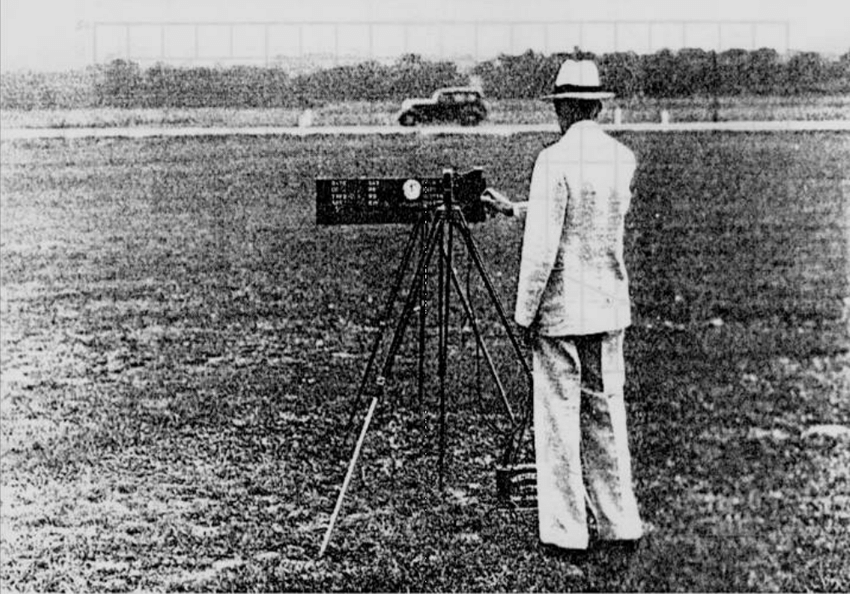
\includegraphics[width=0.6\textwidth]{img/greenshields-experiment.png}
    \caption{Экспериментальная установка Гриншилдса для измерения параметров транспортного потока}
    \label{fig:greenshields-setup}
\end{figure}

Полевой эксперимент проводился с использованием 16-мм кинокамеры, установленной примерно в 350 футах от дороги. Камера делала отдельные снимки через равные промежутки времени. Интервал между кадрами регулировался электрическим приводом и, как правило, выбирался таким образом, чтобы каждый автомобиль попадал как минимум на два последовательных кадра. Почти все серии снимков выполнялись с частотой 88 кадров в минуту. При таком выборе интервала расстояние, пройденное автомобилем между двумя соседними кадрами, численно соответствовало его скорости в милях в час, что существенно упрощало дальнейшую обработку результатов.

\begin{figure}[ht]
    \centering
    \begin{subfigure}[t]{0.48\textwidth}
        \centering
        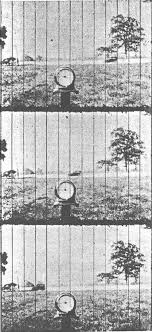
\includegraphics[height=7cm,keepaspectratio]{img/greenshields-experiment-2.jpg}
        \caption{Рис. 4: Три последовательных кадра, снятых на кинокамеру}
    \end{subfigure}
    \hfill
    \begin{subfigure}[t]{0.48\textwidth}
        \centering
        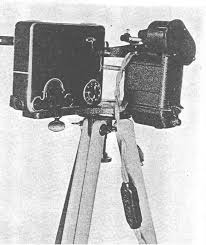
\includegraphics[height=7cm,keepaspectratio]{img/greenshields-experiment-3.jpg}
        \caption{Рис. 5: Кинокамера с моторным приводом, использовавшаяся Гриншилдсом}
    \end{subfigure}
\end{figure}

Территориально эксперименты проводились на различных участках дорог US 20, US 6, US 23 и US 25. Один из участков US 20, пролегающий между городами Норуолк и Монровилл (штат Огайо), представлен на рис.~\ref{fig:monroeville-norwalk}.

\begin{figure}[h]
    \centering
    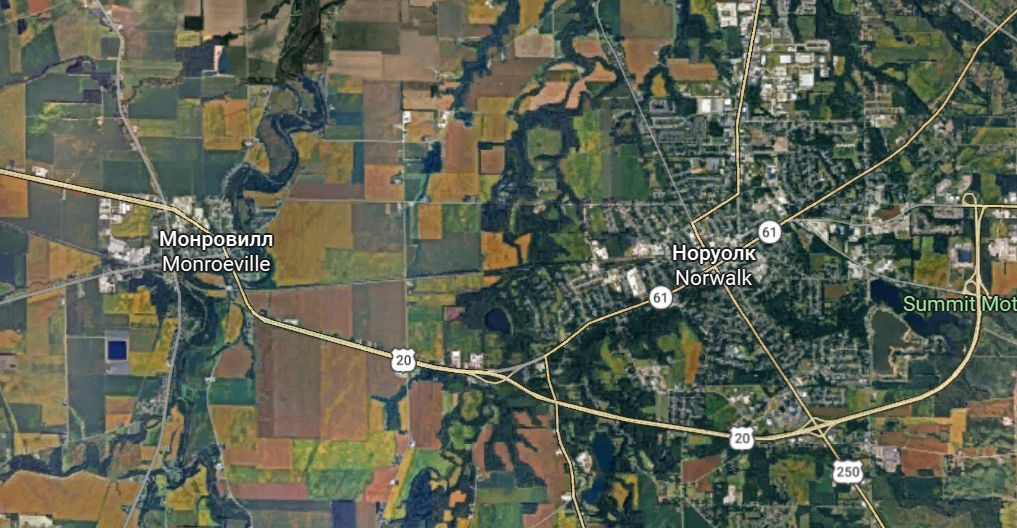
\includegraphics[width=0.6\textwidth]{img/greenshields-experiment-pic.png}
    \caption{Современный спутниковый снимок участка US 20}
    \label{fig:monroeville-norwalk}
\end{figure}


Для исключения сильного смазывания изображения требовалось, чтобы автомобиль находился не ближе примерно 300 футов от камеры. Длина видимого участка дороги на одном кадре составляла около 125 футов. В начале каждой плёнки и затем каждый час в кадр помещалась табличка с указанием места наблюдения, даты, времени, интервала между кадрами, выдержки и другой служебной информации. Для удобства распознавания автомобилей на противоположной стороне дороги натягивалось белое полотно, улучшающее контраст изображения.

Важной частью эксперимента была калибровка масштаба изображения. Для этого использовались либо хорошо различимые неподвижные ориентиры вдоль дороги, например, столбы или другие объекты, либо специальная разметка: вдоль покрытия укладывали 100-футовую ленту и через каждые 10 футов помещали метки, которые фотографировались камерой. Благодаря этому по кадрам можно было достаточно точно восстановить расстояние, пройденное автомобилем за фиксированное время, а значит, определить его скорость.

После съёмки данные переносились в таблицы. Сначала для практически всех автомобилей, прошедших через точку наблюдения, определялись моменты прохождения и скорости. Затем автомобили группировались сначала по десяткам, а затем по сотням, что позволяло строить скользящие средние и уменьшать влияние случайных колебаний. Такой способ обработки был особенно важен, поскольку реальные данные движения всегда содержат разброс, связанный с различиями в поведении водителей, составом потока и дорожными условиями.

Наблюдения выполнялись на нескольких участках дорог штата Огайо. Для участков со свободным движением Гриншилдс получил среднюю свободную скорость порядка $43.5$ миль в час для двухполосных дорог. Далее эта величина использовалась как оценка скорости свободного движения $v_{\max}$.

Главная гипотеза Гриншилдса состояла в том, что средняя скорость потока линейно убывает с ростом плотности:
\begin{equation*}
    V(\rho)=v_{\max}\left(1-\frac{\rho}{\rho_{\max}}\right),
\end{equation*}
где $V(\rho)$ -- средняя скорость при плотности $\rho$, $v_{\max}$ -- скорость свободного движения, $\rho_{\max}$ -- предельная плотность, соответствующая полной остановке потока. Зависимость скорости потока от его плотности схематически приведена на рис.~\ref{fig:greenshields-speed-density}, фундаментальная диаграмма -- на рис.~\ref{fig:greenshields-fundamental-diagram}. Оригинальная фундаментальная диаграмма представлена на рис. ~\ref{fig:greenshields-fundamental-diagram-orig}.

\begin{figure}[h]
    \centering
    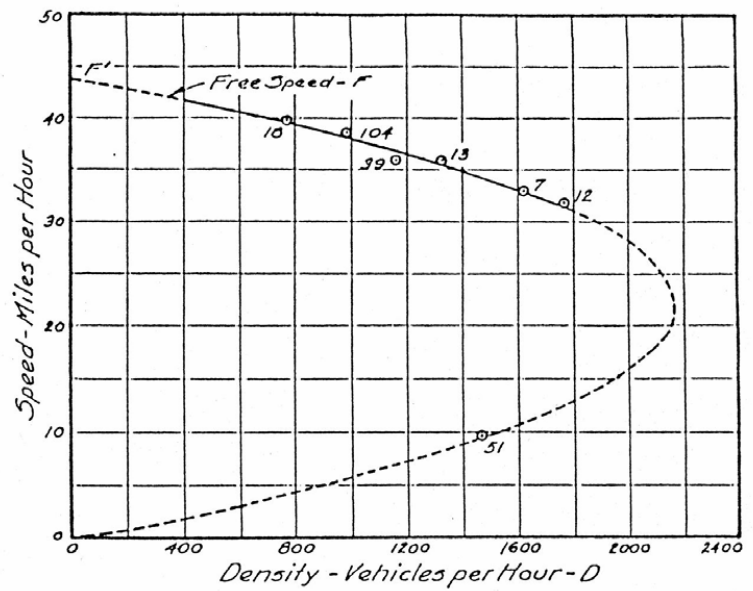
\includegraphics[width=0.6\textwidth]{img/greenshields-fundamental-diagram.png}
    \caption{Фундаментальная диаграмма из оригинальной статьи}
    \label{fig:greenshields-fundamental-diagram-orig}
\end{figure}

Тогда для интенсивности потока $q$ получаем
\begin{equation*}
    q(\rho)=\rho\,V(\rho)=v_{\max} \rho\left(1-\frac{\rho}{\rho_{\max}}\right).
\end{equation*}
Следовательно, зависимость интенсивности от плотности оказывается параболической. Максимум интенсивности достигается при
\begin{equation*}
    \rho=\frac{\rho_{\max}}{2},
    \qquad
    v=\frac{v_{\max}}{2},
    \qquad
    q_{\max}=\frac{v_{\max} \rho_{\max}}{4}.
\end{equation*}

Модель Гриншилдса является простейшей аналитической моделью фундаментальной диаграммы. Линейная зависимость скорости от плотности хорошо подходит как первое приближение, однако реальные экспериментальные данные часто демонстрируют более сложную форму фундаментальной диаграммы, особенно вблизи режима насыщения и в области возникновения заторов. Тем не менее, именно модель Гриншилдса исторически стала отправной точкой для развития более точных и содержательных моделей транспортного потока.

\section{Модель Гринберга}

Модель Гринберга, предложенная в 1959 году, представляет собой подход к описанию динамики транспортных потоков методами механики сплошной среды. Эта модель, в отличие от линейной модели Гриншилдса, лучше описывает поведение потока при высоких плотностях.

Гарольд Гринберг (1928--2016 гг.) --- выдающийся американский математик и специалист по исследованию операций. Помимо своего вклада в дорожную науку, Гринберг сделал блестящую академическую карьеру, став почётным профессором департамента статистики и компьютерных информационных систем Колледжа Баруха (CUNY), где он прославился разработкой элегантных математических алгоритмов для решения сложных логистических задач.

Основная идея состоит в том, что при достаточно больших плотностях транспортный поток можно рассматривать как одномерную сжимаемую среду. Введём субстанциональную производную. В одномерном случае она будет выглядеть следующим образом:
\begin{equation}
\frac{D}{Dt}=\frac{\partial}{\partial t}+v\frac{\partial}{\partial x}.
\label{eq:material_derivative}
\end{equation}
Тогда уравнение движения в модели Гринберга записывается в виде
\begin{equation}
\frac{Dv}{Dt}+\frac{c^2}{\rho}\frac{\partial \rho}{\partial x}=0,
\label{eq:greenberg_motion_material}
\end{equation}
а уравнение неразрывности имеет вид
\begin{equation}
\frac{\partial \rho}{\partial t}+\frac{\partial (\rho v)}{\partial x}=0.
\label{eq:greenberg_continuity}
\end{equation}
Раскрывая производную в \eqref{eq:greenberg_continuity}, получаем
\[
\frac{\partial \rho}{\partial t}+v\frac{\partial \rho}{\partial x}
+\rho\frac{\partial v}{\partial x}=0,
\]
то есть
\begin{equation}
\frac{D\rho}{Dt}+\rho\frac{\partial v}{\partial x}=0.
\label{eq:greenberg_continuity_material}
\end{equation}

Здесь \(c>0\) --- параметр модели, имеющий размерность скорости. Далее предполагается, что скорость зависит только от плотности:
\[
v(x, t)=V(\rho(x, t)).
\]
Тогда вдоль траектории движения выполняется правило цепочки:
\begin{equation}
\frac{Dv}{Dt}=V'(\rho)\frac{D\rho}{Dt}.
\label{eq:chain_material}
\end{equation}
Подставляя \eqref{eq:chain_material} в \eqref{eq:greenberg_motion_material}, имеем
\[
V'(\rho)\frac{D\rho}{Dt}
+\frac{c^2}{\rho}\frac{\partial \rho}{\partial x}=0.
\]
Из уравнения неразрывности \eqref{eq:greenberg_continuity_material} следует
\[
\frac{D\rho}{Dt}=-\rho\frac{\partial v}{\partial x}.
\]
Поэтому
\[
-\rho V'(\rho)\frac{\partial v}{\partial x}
+\frac{c^2}{\rho}\frac{\partial \rho}{\partial x}=0.
\]
Так как \(v(x,t)=V(\rho(x,t))\), то
\[
\frac{\partial v}{\partial x}
=V'(\rho)\frac{\partial \rho}{\partial x}.
\]
Подставляя это выражение, получаем
\[
-\rho\left(V'(\rho)\right)^2\frac{\partial \rho}{\partial x}
+\frac{c^2}{\rho}\frac{\partial \rho}{\partial x}=0.
\]
При нетривиальном распределении плотности \(\frac{\partial \rho}{\partial x}\neq 0\), откуда следует условие совместности
\[
\left(\rho V'(\rho)\right)^2=c^2.
\]

Физически логичным является отрицательный корень, так как скорость должна уменьшаться при росте плотности:
\[
V'(\rho)=-\frac{c}{\rho}.
\]
Интегрируя это соотношение и учитывая, что $V(\rho_{\max})=0$, получаем логарифмический закон Гринберга:
\begin{equation}
\boxed{V(\rho)=c\ln\frac{\rho_{\max}}{\rho}}
\label{eq:greenberg_speed_density}
\end{equation}

\begin{figure}[ht]
\centering
\begin{tikzpicture}
\begin{axis}[
    width=0.6\textwidth,
    height=0.37\textwidth,
    xmin=0, xmax=1,
    ymin=0, ymax=4,
    xlabel={$\rho/\rho_{\max}$},
    ylabel={$v/c$},
    grid=both,
    legend style={at={(0.97,0.97)},anchor=north east},
    samples=200,
    domain=0.02:0.999
]
\addplot[thick] {ln(1/x)};
\end{axis}
\end{tikzpicture}
\caption{Нормированная зависимость скорости от плотности потока в модели Гринберга}
\label{fig:greenberg_speed_general}
\end{figure}
Тогда фундаментальная диаграмма имеет вид:
\begin{equation}
Q(\rho)=q(\rho)=\rho\,V(\rho)
=c\rho\ln\frac{\rho_{\max}}{\rho}.
\label{eq:greenberg_fundamental}
\end{equation}
Из формулы \eqref{eq:greenberg_fundamental} видно, что
\[
q(\rho)\to 0 \; \text{при} \; \rho\to 0
\;\text{и}\;
q(\rho)=0 \; \text{при} \; \rho=\rho_{\max}.
\]
Следовательно, поток мал как при очень разреженном движении, так и вблизи полного затора. Между этими двумя режимами существует максимум. Найдём точку максимума:
\[
\frac{dq}{d\rho}
=c\left(\ln\frac{\rho_{\max}}{\rho}-1\right)=0.
\]
Отсюда
\[
\rho_*=\frac{\rho_{\max}}{e}.
\]
Соответствующая скорость равна
\[
V(\rho_*)=c.
\]
Таким образом, параметр $c$ допускает наглядную физическую интерпретацию: он соответствует значению скорости, при которой достигается максимальная интенсивность транспортного потока.

Логарифмический закон \eqref{eq:greenberg_speed_density} хорошо передаёт поведение плотного потока: при увеличении плотности скорость убывает всё сильнее, а при приближении к плотности затора стремится к нулю. Вместе с тем модель имеет известное ограничение: при \(\rho\to 0\) формально получается \(v\to\infty\), поэтому её нельзя считать адекватной моделью свободного, очень разреженного движения.

\begin{figure}[ht]
\centering
\begin{tikzpicture}
\begin{axis}[
    width=0.6\textwidth,
    height=0.37\textwidth,
    xmin=0, xmax=1,
    ymin=0, ymax=0.40,
    xlabel={$\rho/\rho_{\max}$},
    ylabel={$q/(c\rho_{\max})$},
    grid=both,
    samples=200,
    domain=0.001:0.999
]
\addplot[thick] {x*ln(1/x)};
\end{axis}
\end{tikzpicture}

\captionsetup{justification=centering}
\caption{Нормированная фундаментальная диаграмма Гринберга:
\\
\(\displaystyle \frac{q}{c\rho_{\max}}=\frac{\rho}{\rho_{\max}}\ln\frac{\rho_{\max}}{\rho}\).}
\label{fig:greenberg_normalized}
\end{figure}

Свою математическую модель Гринберг проверил с помощью ряда экспериментов. Если ввести пространственный интервал между автомобилями \(h\), то при измерении в футах и плотности
в автомобилях на милю
\[
h=\frac{5280}{\rho}.
\]
Из \eqref{eq:greenberg_speed_density} тогда следует
\[
h=h_{\min} e^{v/c},
\quad
h_{\min}=\frac{5280}{\rho_{\max}}.
\]
Значит, эксперимент можно свести к подгонке прямой в координатах \(v\) и \(\ln h\) методом наименьших квадратов.

В первом эксперименте использовались измерения, выполненные в северной трубе туннеля Линкольна (Нью-Йорк). Современный вид туннеля представлен на рис.~\ref{fig:lincoln-tunnel}. На коротком участке дороги была установлена машина Simplex Productograph. Работали два наблюдателя: один стоял у входа в измеряемую зону, другой -- у выхода из неё. При прохождении автомобиля через каждую из двух точек фиксировалось время. Такая схема позволяла достаточно точно определить скорость каждого автомобиля, а также пространственный интервал между автомобилями.

\begin{figure}[h]
    \centering
    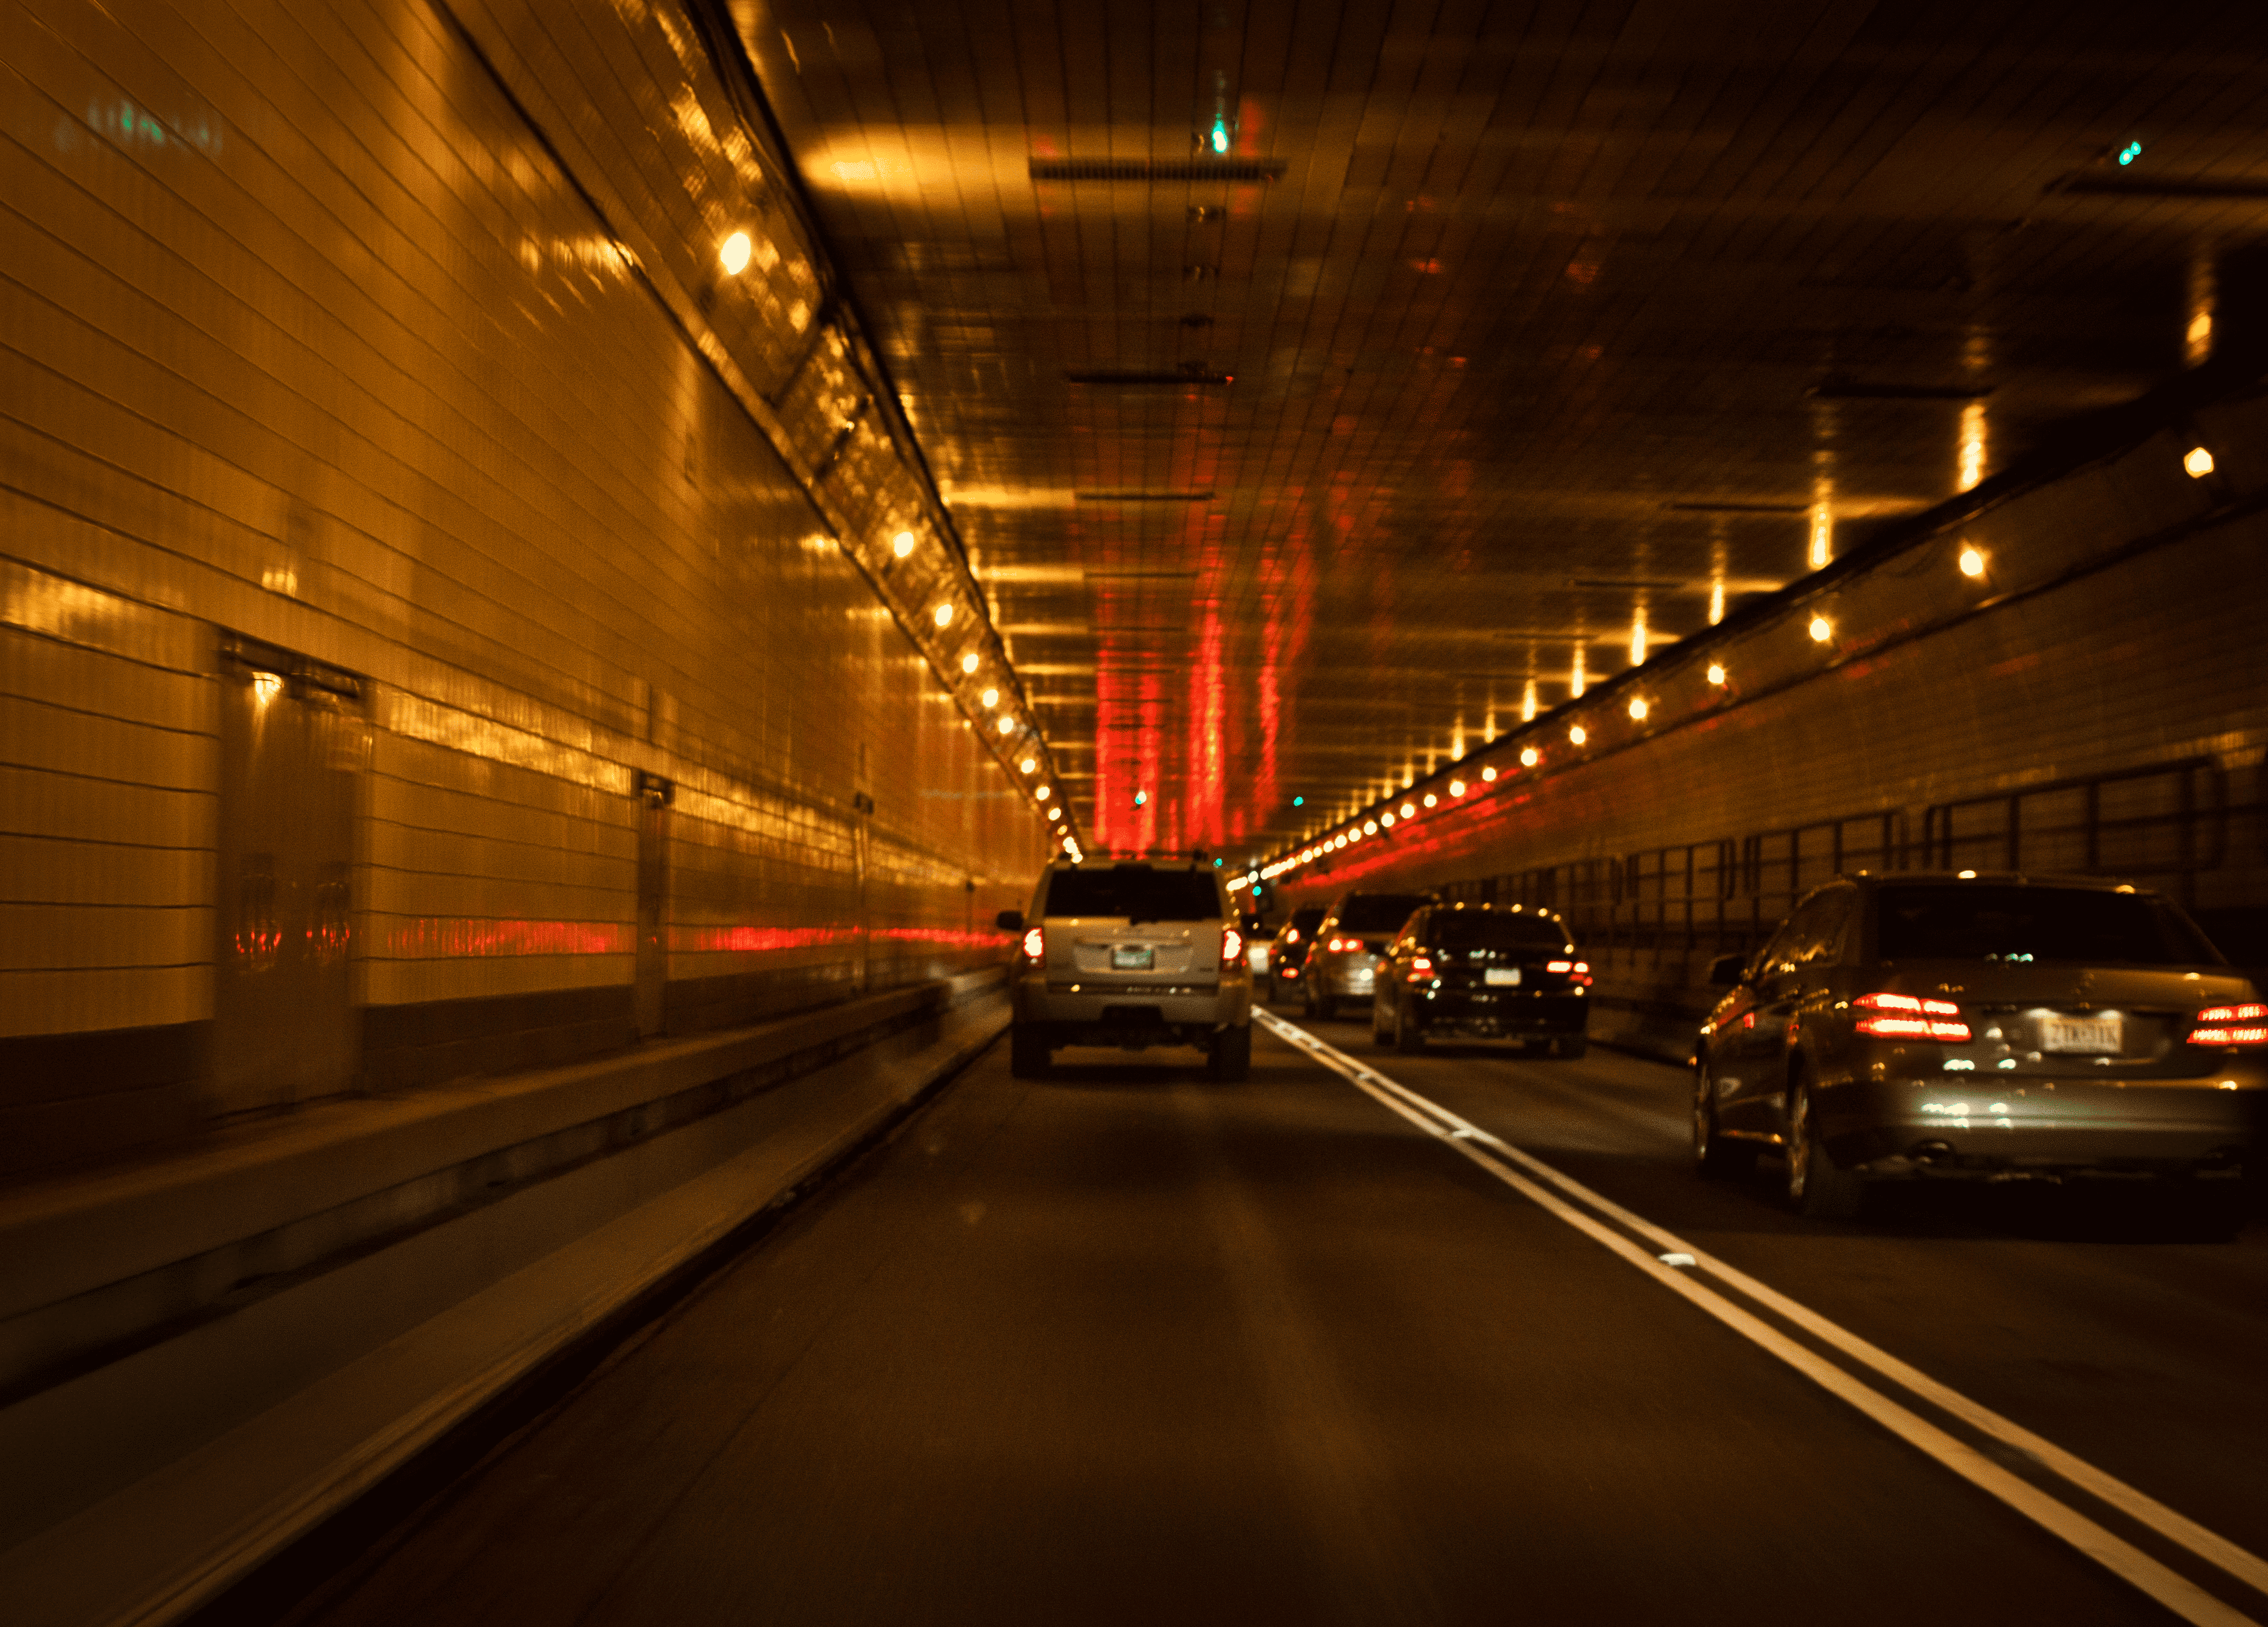
\includegraphics[width=0.6\textwidth]{img/lincoln-tunnel.png}
    \caption{Современный вид туннеля Линкольна (Нью-Йорк)}
    \label{fig:lincoln-tunnel}
\end{figure}

После этого данные разбивались на классы скоростей, и для каждого класса вычислялся средний интервал \(h\). Именно эти усреднённые значения затем использовались при подгонке модели. Для туннеля Линкольна Гринберг получил соотношения
\begin{equation*}
h(v)=23.2\,e^{v/17.2},
\label{eq:lincoln_h}
\end{equation*}
или, что то же самое,
\begin{equation*}
\rho(v)=228\,e^{-v/17.2}.
\label{eq:lincoln_rho}
\end{equation*}
Следовательно,
\begin{equation*}
v(\rho)=17.2\ln\frac{228}{\rho},
\quad
q(\rho)=17.2\,\rho\ln\frac{228}{\rho}.
\label{eq:lincoln_greenberg}
\end{equation*}

Зависимость скорости от плотности потока, приведённая в оригинальной статье, представлена на рис.~\ref{fig:greenberg-vrho}.

\begin{figure}[ht]
    \centering
    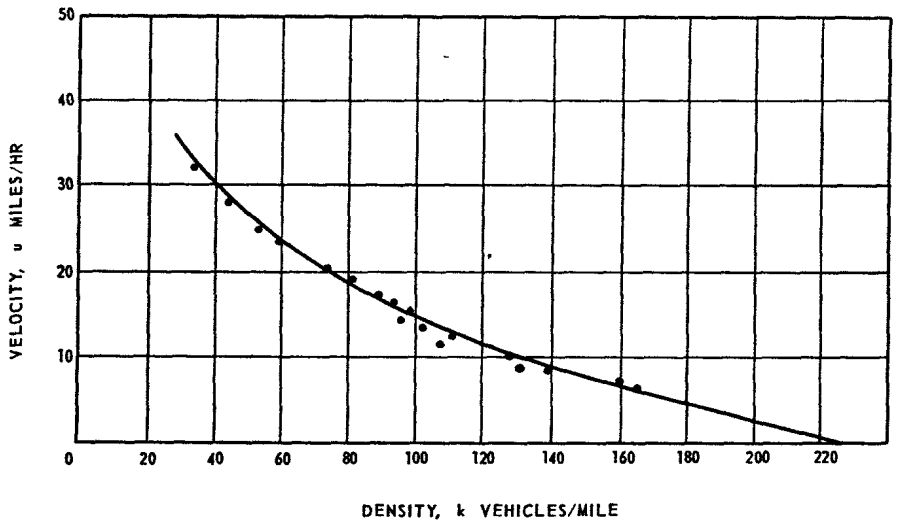
\includegraphics[width=0.8\textwidth]{img/greenberg-velocity-density.png}
    \caption{Зависимость скорости потока от плотности в оригинальной статье}
    \label{fig:greenberg-vrho}
\end{figure}

Данные второго эксперимента представляли собой пятиминутные усреднённые показатели трассы Мерритт-Паркуэй. Для каждого интервала вычислялись средние значения скорости и дистанции между машинами. За счёт временного усреднения эти данные характеризуются меньшей зашумленностью, чем результаты прямых наблюдений в первом эксперименте.

Метод наименьших квадратов приводит к формулам
\begin{equation*}
h(v)=24.6\,e^{v/16.1},
\label{eq:merritt_h}
\end{equation*}
или
\begin{equation*}
\rho(v)=215\,e^{-v/16.1}.
\label{eq:merritt_rho}
\end{equation*}
Отсюда
\begin{equation*}
v(\rho)=16.1\ln\frac{215}{\rho},
\quad
q(\rho)=16.1\,\rho\ln\frac{215}{\rho}.
\label{eq:merritt_greenberg}
\end{equation*}

Несмотря на различие в способе усреднения данных, форма полученной кривой оказывается той же самой. Меняются только параметры, то есть конкретные значения \(c\) и \(\rho_{\max}\), зависящие от свойств данного дорожного участка.

Отдельно Гринберг исследует поведение потока вблизи узких мест (bottlenecks). Пропускная способность узкого места начинает определять режим потока как перед ним, так и после него. Если входной поток меньше уровня, который может пропустить узкое место, движение определяется в основном свойствами самого дорожного участка. Если же этот уровень превышен, возникает растущая очередь, и режим движения
становится контролируемым узким местом.

Модель Гринберга хорошо описывает плотный поток и режимы, близкие к затору. В то же время, модель плохо подходит для очень малых плотностей, где логарифмическая формула предсказывает неограниченный рост скорости.
\section{Модель Нагеля-Шрекенберга}
Модель Нагеля-Шрекенберга (1992 г.) относится к моделям клеточных автоматов. В таких моделях дорога разбивается на клетки, время также считается дискретным. Часто считается, что в клетке может находиться не больше одного АТС. Таким образом, получаются разностные аналоги рассматриваемых ранее макроскопических уравнений. Кроме того, в таких моделях множество возможных значений скорости АТС также часто принимается дискретным.

Кай Нагель, ныне профессор Технического университета Берлина, специализируется на крупномасштабных многоагентных симуляциях транспортных систем (проект MATSim) и методах параллельных вычислений. Михаэль Шрекенберг, занимающий пост профессора в Университете Дуйсбурга—Эссена, посвятил свою карьеру физике транспорта, логистике и моделированию толпы, став одним из ведущих экспертов по управлению дорожным движением и прогнозированию «фантомных пробок».

В рамках модели дорога представляется в виде одномерной цепочки из \(L\) ячеек одинаковой длины. Каждая ячейка либо свободна, либо занята ровно одним автомобилем. Скорость каждого автомобиля принимает целые значения от \(0\) до \(v_{\max}\).

Пусть \(x_n(t)\) обозначает положение \(n\)-го автомобиля в момент времени \(t\), \(v_n(t)\) -- его скорость, а \(d_n(t)\) -- число свободных ячеек перед ним до следующего автомобиля. Тогда за один шаг времени \(\Delta t = 1\) состояние всех АТС в системе обновляется в соответствии со следующими правилами. Сначала выполняется ускорение:
\[
v_n \rightarrow \min\{v_n+1,\;v_{\max}\}.
\]
Затем учитывается необходимость торможения из-за впереди идущего автомобиля:
\[
v_n \rightarrow \min\{v_n,\;d_n\}.
\]
После этого вводится случайное возмущение для учета различий в поведении АТС:
\[
v_n \rightarrow 
\begin{cases} 
\max\{v_n - 1, 0\} & \text{с вероятностью } p, \\
v_n & \text{с вероятностью } 1 - p,
\end{cases}
\]
Наконец, после пересчёта скоростей происходит перемещение автомобилей:
\[
x_n \rightarrow x_n+v_n.
\]
Все четыре приведенных шага необходимы для воспроизведения основных свойств транспортного потока. Так, например, шаг 3 учитывает неустойчивость транспортного потока при достаточно больших плотностях. Кроме того, случайный шаг делает модель содержательной с физической точки зрения. Без него движение быстро переходило бы в слишком правильный и искусственный режим, тогда как в реальном транспортном потоке неизбежно присутствуют случайные замедления, различия в реакции водителей и мелкие внешние возмущения.

Численный эксперимент, описанный в статье, проводился методом Монте-Карло. В основной серии расчётов авторы рассматривали движение на однополосной дороге с периодическими граничными условиями, то есть на кольце. Такая постановка удобна тем, что число автомобилей в системе остаётся постоянным. Если в системе находится \(N\) автомобилей, то средняя плотность задаётся формулой
\[
\rho=\frac{N}{L}.
\]
Для каждого фиксированного значения плотности авторы брали случайное начальное расположение автомобилей, причём начальные скорости полагались равными нулю. После этого модель некоторое время эволюционировала без измерений, чтобы система успела выйти в стационарный режим. Лишь после этапа релаксации начинался сбор статистики.

Существенно, что измерение характеристик потока было организовано так, чтобы оно напоминало реальные дорожные наблюдения. Вместо того, чтобы определять плотность только как отношение \(N/L\), авторы вводили усреднённую по времени локальную плотность на фиксированной ячейке:
\[
\bar{\rho}^{\,T}(i)=\frac{1}{T}\sum_{t=t_0+1}^{t_0+T} n_i(t),
\]
где
\[
n_i(t)=
\begin{cases}
1, & \text{если ячейка } i \text{ занята в момент } t,\\
0, & \text{если ячейка } i \text{ свободна.}
\end{cases}
\]
При этом $\lim_{T \to \infty}\bar{\rho}^{\,T} = \rho$. Аналогично усреднённый по времени поток между соседними ячейками \(i\) и \(i+1\) определялся формулой
\[
\bar{q}^{\,T}(i,i+1)=\frac{1}{T}\sum_{t=t_0+1}^{t_0+T} n_{i,i+1}(t),
\]
где $n_{i,i+1}(t)=1$, если за шаг времени автомобиль пересёк границу между i и i+1 и $n_{i,i+1}(t)=0$ иначе.

Модель была реализована на языке FORTRAN, а расчёты выполнялись как на рабочей станции IBM RS/6000 320H, так и на многопроцессорной системе iPSC-860 Hypercube. Основные серии моделирования проводились при \(v_{\max}=5\), поскольку именно это значение авторы считали наиболее реалистичным для качественного описания движения на автомагистрали.

Результаты эксперимента оказались весьма показательными. При малой плотности движение остаётся почти невозмущённым: автомобили движутся свободно, практически не мешая друг другу, а поток \(q\) растёт с увеличением плотности \(\rho\), как показано на рис.~\ref{fig:nagel_free_flow}. На нём представлена пространственно-временная диаграмма: по горизонтали отложено пространство, по вертикали -- время, пустые ячейки отмечены точками, а занятые -- числами, равными текущим скоростям автомобилей.

\begin{figure}[ht!]
    \centering
    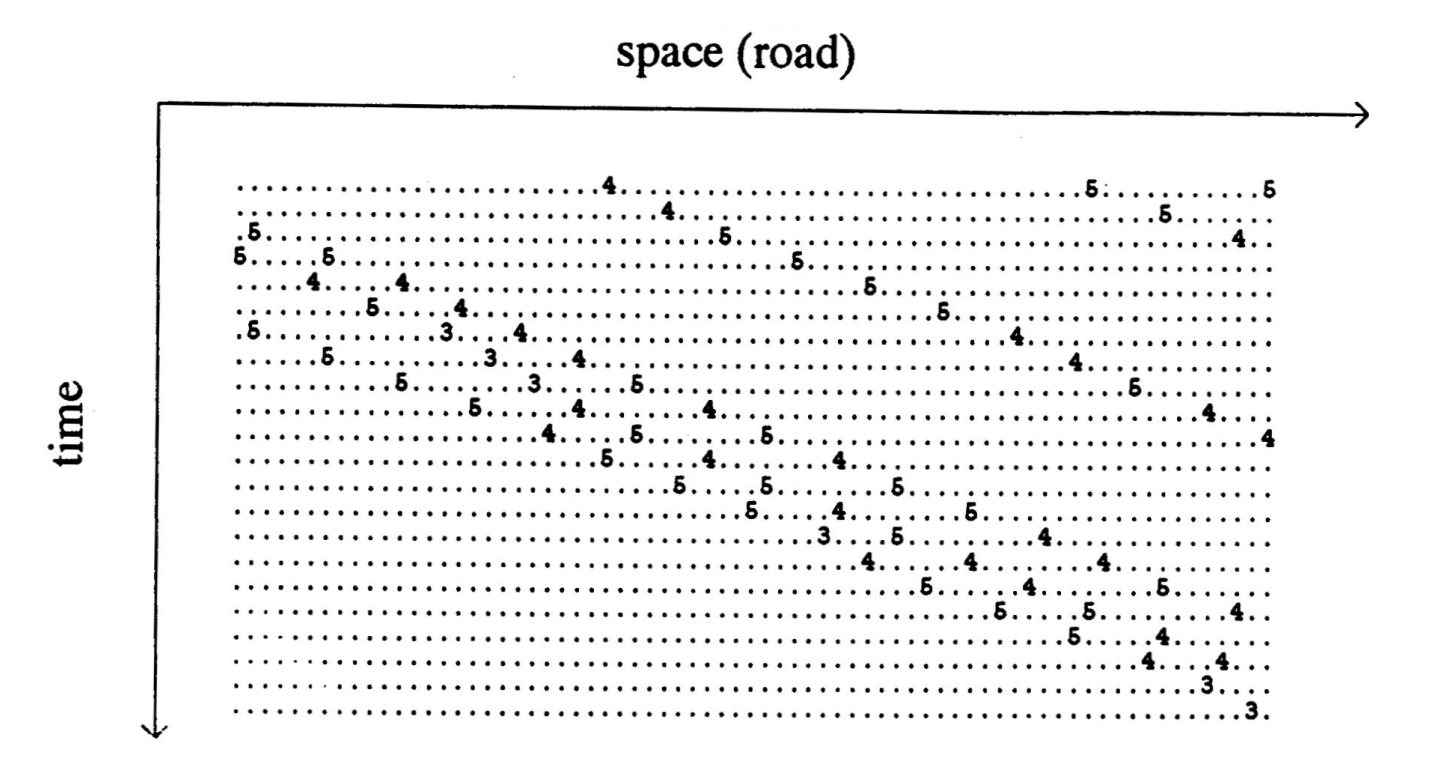
\includegraphics[width=0.75\textwidth]{img/nagel-sch-1.png}
    \caption{Диаграмма режима свободного движения}
    \label{fig:nagel_free_flow}
\end{figure}

При увеличении плотности возникают локальные скопления автомобилей, которые затем перерастают в пробки. Это проиллюстрировано на рис.~\ref{fig:nagel_jam}. На этой диаграмме хорошо заметно, что область затора движется в сторону, противоположную направлению движения автомобилей. Иными словами, сами машины едут вперёд, а волна уплотнения распространяется назад. Отдельный автомобиль подъезжает к такой области с достаточно высокой скоростью, затем тормозит почти до полной остановки, некоторое время продвигается медленно внутри плотного кластера, а после выхода из него снова разгоняется. На рис.~\ref{fig:nagel_aerophoto} представлены траектории движения автомобилей по данным аэрофотосъёмки. Каждая линия соответствует одному АТС.

\begin{figure}[ht!]
    \centering
    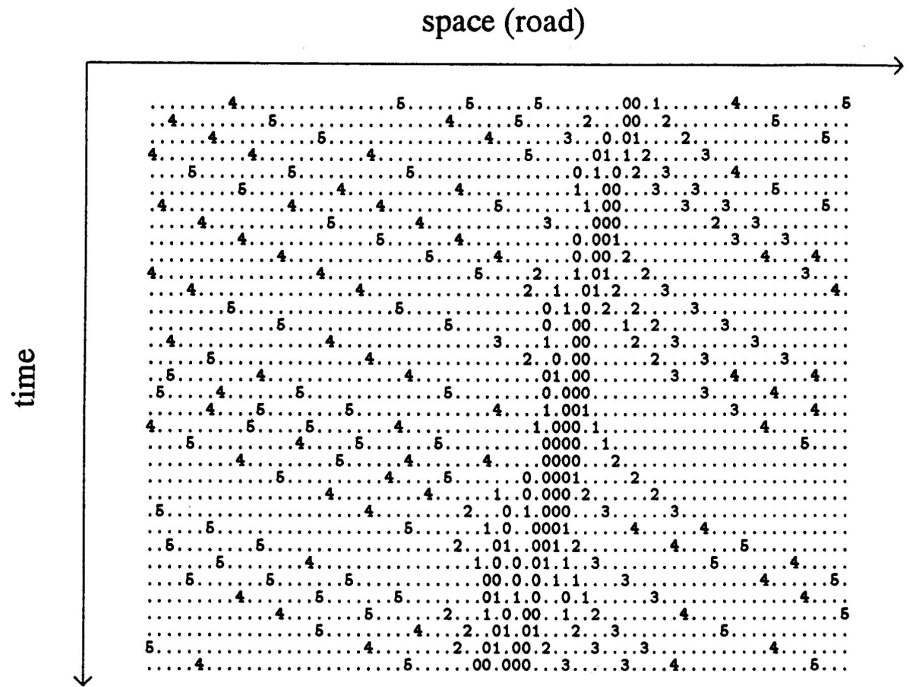
\includegraphics[width=0.75\textwidth]{img/nagel-sch-2.png}
    \caption{Пространственно-временная диаграмма при повышенной плотности. Видно формирование затора и его распространение против направления движения автомобилей.}
    \label{fig:nagel_jam}
\end{figure}

\begin{figure}[ht!]
    \centering
    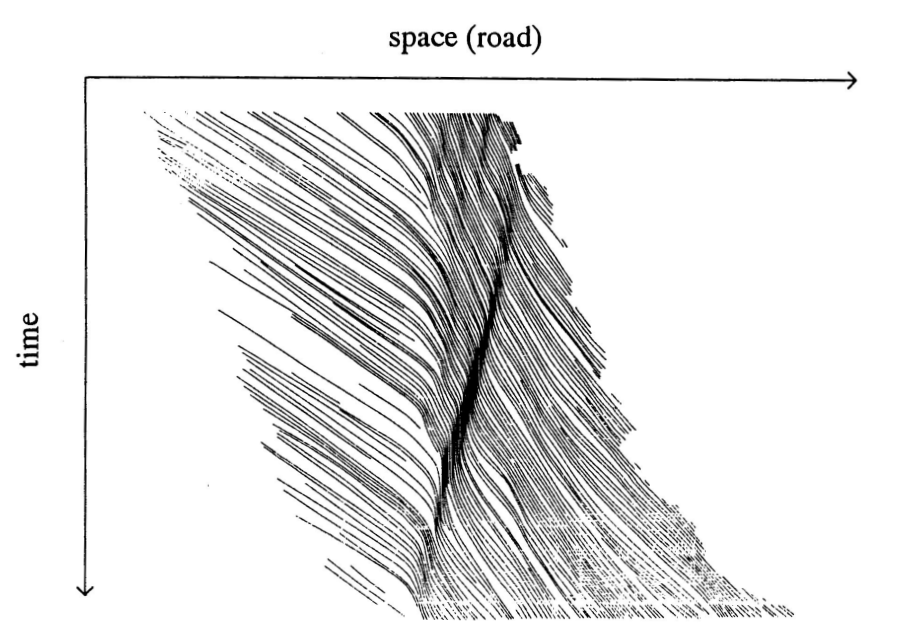
\includegraphics[width=0.75\textwidth]{img/nagel-sch-3.png}
    \caption{Пространственно-временные траектории автомобилей по данным аэрофотосъёмки}
    \label{fig:nagel_aerophoto}
\end{figure}

На рис.~\ref{fig:nagel_orig_diagram} представлена фундаментальная диаграмма, полученная авторами модели. Эта зависимость имеет типичную для транспортных потоков форму: сначала поток возрастает, затем достигает максимума, после чего начинает уменьшаться. Однако после достижения некоторой критической области дальнейшее увеличение плотности уже не усиливает поток, а, наоборот, разрушает свободный режим движения и приводит к падению пропускной способности. Авторы отмечают, что смена режима происходит примерно вблизи \(\rho \approx 0.08\).

\begin{figure}[ht!]
    \centering
    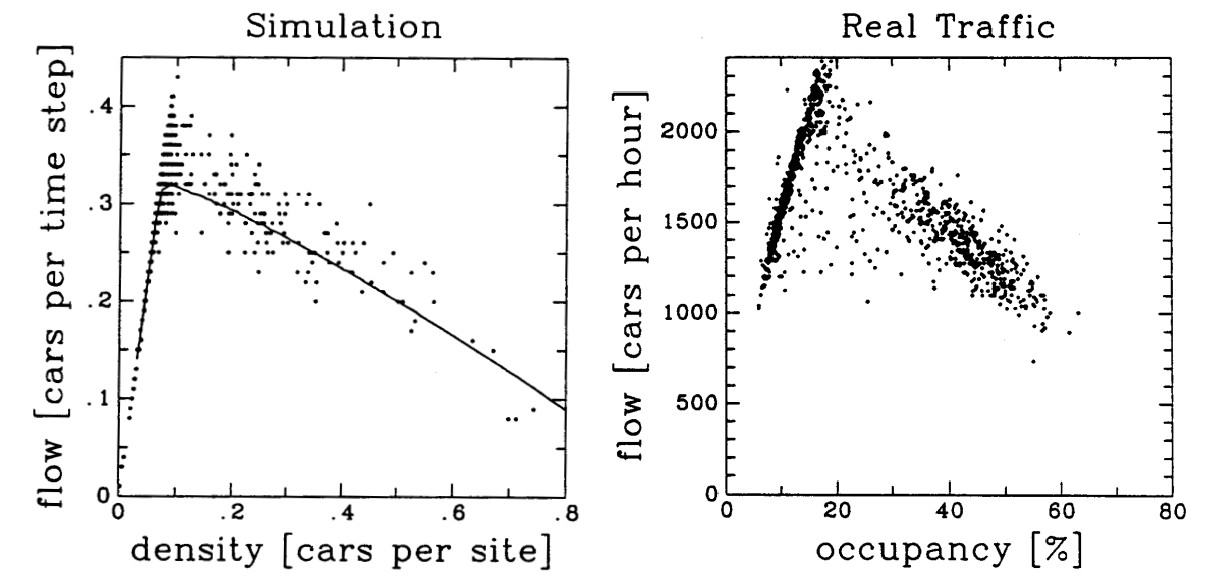
\includegraphics[width=1\textwidth]{img/nagel-sch-4.png}
    \caption{Зависимость потока от плотности в симуляции (слева) и потока от занятости полосы (occupancy) в реальных дорожных данных (справа)}
    \label{fig:nagel_orig_diagram}
\end{figure}

Полученная в эксперименте зависимость \(q=Q(\rho)\) может быть приближенно описана формулой~\ref{eq:nagel_formula}, а фундаментальную диаграмму можно изобразить как показано на рис.~\ref{fig:nagel_diagram_tikhonov}.
\begin{equation}
Q(\rho)=
\begin{cases}
k_1 \rho, & 0 \le \rho \le \rho^*, \\[4pt]
k_2(\rho_{\max}-\rho), & \rho^* \le \rho \le \rho_{\max}.
\end{cases}
\label{eq:nagel_formula}
\end{equation}

\begin{figure}
\centering
\begin{tikzpicture}
    \def\rhostar{3.0}
    \def\rhomax{8.0}
    \def\qmax{3.2}

    % axes
    \draw[->] (-0.2,0) -- (\rhomax+0.9,0) node[right] {$\rho$};
    \draw[->] (0,-0.2) -- (0,\qmax+1.0) node[above] {$q$};

    % graph
    \draw[thick] (0,0) -- (\rhostar,\qmax) -- (\rhomax,0);

    % dashed lines
    \draw[dashed] (\rhostar,0) -- (\rhostar,\qmax);
    \draw[dashed] (0,\qmax) -- (\rhostar,\qmax);

    % points
    \fill (0,0) circle (1.4pt);
    \fill (\rhostar,\qmax) circle (1.4pt);
    \fill (\rhostar,0) circle (1.4pt);
    \fill (\rhomax,0) circle (1.4pt);

    % labels
    \node[below left] at (0,0) {$0$};
    \node[left] at (0,\qmax) {$q_{\max}$};
    \node[below] at (\rhostar,0) {$\rho^*$};
    \node[below] at (\rhomax,0) {$\rho_{\max}$};

\end{tikzpicture}
\caption{Фундаментальная диаграмма в модели Нагеля-Шрекенберга}
\label{fig:nagel_diagram_tikhonov}
\end{figure}

Коэффициенты \(k_1>0\), \(k_2>0\) -- это некие скорости
(точнее, величины, имеющие размерность скорости). При этом
\[
k_1 \rho^* = k_2(\rho_{\max}-\rho^*)
\quad \Longrightarrow \quad
k_2 = k_1 \frac{\rho^*}{\rho_{\max}-\rho^*}.
\]

Выразим из (\ref{eq:nagel_formula}) закон безопасного движения:
\[
v = V(\rho) = \frac{Q(\rho)}{\rho} =
\begin{cases}
k_1, & 0 < \rho \le \rho^*, \\[6pt]
k_2\left(\dfrac{\rho_{\max}}{\rho}-1\right), & \rho^* \le \rho \le \rho_{\max}.
\end{cases}
\]

Характер движения разбивается на две фракции:
\[
\begin{aligned}
1)\;& 0 \le \rho \le \rho^*
\text{ -- свободное движение, }
\Longrightarrow V(\rho)=v_{\max}\;(=k_1). \\[4pt]
2)\;& \rho^* \le \rho \le \rho_{\max}
\text{ -- затруднённое движение, }
\Longrightarrow V(\rho)\downarrow\downarrow\ \text{по гиперболе.}
\end{aligned}
\]

Окончательно получаем
\[
V(\rho)=
\begin{cases}
v_{\max}, & 0 < \rho \le \rho^*, \\[8pt]
\dfrac{v_{\max}\rho^*}{\rho_{\max}-\rho^*}
\left(\dfrac{\rho_{\max}}{\rho}-1\right),
& \rho^* \le \rho \le \rho_{\max}.
\end{cases}
\]

Здесь \(\rho=\rho^*\) -- переходная плотность от свободного движения к затруднённому. Зависимость скорости потока от его плотности представлена на рис.~\ref{fig:nagel_vrho}.

\begin{figure}[ht!]
\begin{center}
\begin{tikzpicture}
    \def\rhostar{3.0}
    \def\rhomax{8.0}
    \def\vmax{3.0}
    \pgfmathsetmacro{\coef}{\vmax*\rhostar/(\rhomax-\rhostar)}

    % axes
    \draw[->] (-0.2,0) -- (\rhomax+1.3,0) node[right] {$\rho$};
    \draw[->] (0,-0.2) -- (0,\vmax+1.1) node[above] {$v$};

    % constant part
    \draw[thick] (0,\vmax) -- (\rhostar,\vmax);

    % open circle at rho = 0
    \draw[fill=white] (0,\vmax) circle (2pt);

    % dashed line
    \draw[dashed] (\rhostar,0) -- (\rhostar,\vmax);

    % hyperbola fragment
    \draw[thick, domain=\rhostar:\rhomax, smooth, variable=\x]
        plot (\x, {\coef*(\rhomax/\x - 1)});

    % point at rho_max
    \fill (\rhomax,0) circle (1.4pt);

    % labels
    \node[left] at (0,\vmax) {$k_1 = v_{\max}$};
    \node[below] at (\rhostar,0) {$\rho^*$};
    \node[below] at (\rhomax,0) {$\rho_{\max}$};

    % annotation
    \node[right] at (5.7,2.3) {фрагмент гиперболы};
    \draw[->] (5.9,2) -- (4.9,1.25);
\end{tikzpicture}
\caption{Зависимость скорости потока от плотности в модели Нагеля-Шрекенберга}
\label{fig:nagel_vrho}
\end{center}
\end{figure}

\section{Современные направления развития моделей фундаментальной диаграммы}
С 1990-х годов развитие моделей фундаментальной диаграммы транспортного потока $Q(\rho)$ велось в рамках двух основных подходов. С одной стороны, исследователи продолжали разрабатывать аналитические зависимости между $\rho$, $v$ и $q$, стремясь сделать их более адаптивными и точными в описании наблюдаемых данных. С другой стороны, возрос интерес к моделям, опирающимся на микроскопические механизмы движения: правила следования за лидером, клеточные автоматы, а впоследствии -- агрегированные сетевые представления. В современных обзорах особо отмечается, что эти направления долгое время развивались параллельно: в то время как одни авторы фокусировались на поиске удобной функциональной формы $Q(\rho)$, другие стремились обосновать её теоретически.

Характерным примером в этом отношении является работа Г.~Ньюэлла (2002 г.), в которой предложена предельно лаконичная модель следования за лидером: траектория ведомого автомобиля практически повторяет траекторию лидера со сдвигом по временной и пространственной осям. Значимость этой идеи заключается в том, что вместо описания сложной динамики ускорений и реакций поведение потока характеризуется всего двумя величинами --- временным и пространственным сдвигами. В стационарном режиме такая схема обуславливает линейную связь между дистанцией и скоростью, что определяет вид фундаментальной диаграммы $Q(\rho)$: после достижения максимума поток $q$ убывает практически линейно с ростом плотности $\rho$. Ценность модели Ньюэлла заключается не столько в самой функциональной форме, сколько в демонстрации возможности вывода макроскопической диаграммы из элементарного микроскопического правила. Это стало важным шагом к созданию физически интерпретируемых и математически строгих моделей. В аналогичном ключе развивались модели оптимальной скорости, в частности модель Бандо, где скорость автомобиля напрямую связывается с дистанцией до лидера. Ключевая концепция здесь иная: водитель стремится к некоторой «желаемой» скорости, определяемой текущим интервалом, а сама зависимость выбирается гладкой для адекватного описания перехода от свободного движения к затору.

Следующий значимый этап связан с работами Х.~М.~дель Кастильо. В середине 1990-х годов он фактически сформулировал аксиоматический подход: роль $Q(\rho)$ может играть не любая аппроксимирующая кривая, а лишь та, которая обладает определенным набором свойств -- корректным поведением в точках максимальной плотности, наличием выраженного максимума и параметрами, имеющими понятную физическую интерпретацию. На основе этих принципов были разработаны обобщенные семейства зависимостей, включающие ранние модели как частные случаи. Позднее дель Кастильо предложил новые функциональные формы, включая модель отрицательной степени (negative power model). Её основная идея состоит в сочетании гибкости гладкой аналитической функции с возможностью аппроксимации кусочно-линейной (треугольной) диаграммы, которая наиболее эффективна в прикладных расчётах.

Особого внимания заслуживает переход к анализу транспортных систем городского масштаба. Работа Н.~Геролиминиса и К.~Даганзо (2008 г.) стала одной из ключевых, поскольку в ней идея фундаментальной диаграммы была перенесена с уровня отдельного участка дороги на уровень городской сети. На измерениях, полученных в городе Иокогама (Япония) авторы сначала показали, что данные отдельных детекторов действительно обладают заметным разбросом, однако после агрегирования по достаточно однородной области этот разброс существенно уменьшается и возникает устойчивая макроскопическая фундаментальная диаграмма. При этом сами авторы подчеркивают, что по одним только стационарным детекторам нельзя окончательно судить о состоянии всей сети, поскольку детекторы характеризуют лишь условия вблизи своих точек установки. Поэтому анализ был дополнен данными GPS-такси, что позволило оценить средние характеристики движения уже для всей исследуемой области и подтвердить существование гладкой зависимости между усредненными параметрами потока на городском уровне.

Содержательно это означает, что для достаточно однородного городского района между средней плотностью $\rho$, средней скоростью $v$ и потоком $q$ вновь проявляется упорядоченная зависимость, хотя на уровне отдельных звеньев сети она может быть скрыта сильным разбросом наблюдений. Более того, в этой работе важную роль играет не только сама диаграмма, но и связанная с ней зависимость между совокупным потоком в сети и скоростью завершения поездок. Именно поэтому макроскопическая фундаментальная диаграмма рассматривается авторами не просто как удобное описание данных, а как основа для управления перегруженной городской сетью. На основе этой модели был предложен способ оптимального управления светофорами и въездами на магистрали, а также способ «оптимального разрыхления» однородного потока АТС на магистрали (с помощью светофоров) с целью уменьшения среднего времени в пути.

Наконец, ключевой тенденцией последних лет стал отказ от жестких параметрических структур в пользу гибких непараметрических и полуэмпирических подходов. В современных сравнительных исследованиях выделяется модель Суна (Sun, 2014 г.), использующая монотонные штрафуемые B-сплайны для аппроксимации $Q(\rho)$. Смысл этого подхода в том, что форма диаграммы в значительной степени определяется самими данными, а степень сглаживания подбирается автоматически. Это особенно удобно потому, что реальные диаграммы часто имеют сложную форму, плохо укладываются в одну простую параметрическую кривую и могут отражать несколько режимов движения. Современные обзоры показывают, что именно такие гибкие модели сегодня лучше всего работают на больших массивах эмпирических наблюдений. Вместе с тем подчеркивается, что дальнейший прогресс связан не только с построением новых форм $Q(\rho)$, но и с более реалистичным учетом разброса данных: реальные наблюдения содержат переходные режимы, гистерезис и неоднородный шум, поэтому дальнейшее развитие темы, по-видимому, будет связано с сочетанием гибких моделей фундаментальной диаграммы и более точных стохастических моделей самого транспортного потока.


\begin{thebibliography}{99}

\bibitem{lectures_mme}
Тихонов Иван Владимирович. Лекции по курсу Математические модели в естествознании.

\bibitem{gasnikov2013}
Введение в математическое моделирование транспортных потоков :
учебное пособие для студентов вузов по направлению
«Прикладные математика и физика» /
[А.~В.~Гасников и др.] ; под ред. А.~В.~Гасникова. --- 2-е изд., испр. и доп. ---
М. : МЦНМО, 2013. --- 426~с. --- ISBN 978-5-4439-0040-7. ---
В реферате использованы с.~23--28, 53.

\bibitem{kuhne2008}
K\"uhne R.~D.
Foundations of Traffic Flow Theory I: Greenshields' Legacy -- Highway Traffic //
Symposium on the Fundamental Diagram: 75 Years
(Greenshields 75 Symposium), July 8--10, 2008, Woods Hole, MA. Preprints. ---
Washington, DC : Transportation Research Board, 2008. --- 8~p.

\bibitem{greenshields1935}
Greenshields B.~D., Bibbins J.~R., Channing W.~S., Miller H.~H.
A Study of Traffic Capacity //
Proceedings of the Highway Research Board. --- 1935. --- Vol.~14. --- P.~448--477.

\bibitem{greenberg1959}
Greenberg H.
An Analysis of Traffic Flow //
Operations Research. --- 1959. --- Vol.~7, no.~1. --- P.~79--85. ---
DOI: \href{https://doi.org/10.1287/opre.7.1.79}{10.1287/opre.7.1.79}.

\bibitem{nagel1992}
Nagel K., Schreckenberg M.
A cellular automaton model for freeway traffic //
Journal de Physique I. --- 1992. --- Vol.~2, no.~12. --- P.~2221--2229. ---
DOI: \href{https://doi.org/10.1051/jp1:1992277}{10.1051/jp1:1992277}.

\bibitem{bramich2022}
Bramich D.~M., Men\'endez M., Amb\"uhl L.
Fitting Empirical Fundamental Diagrams of Road Traffic:
A Comprehensive Review and Comparison of Models Using an Extensive Data Set //
IEEE Transactions on Intelligent Transportation Systems. --- 2022. --- Vol.~23, no.~9. ---
P.~14104--14127. ---
DOI: \href{https://doi.org/10.1109/TITS.2022.3142255}{10.1109/TITS.2022.3142255}.

\bibitem{newell2002}
Newell G.~F.
A simplified car-following theory: a lower order model //
Transportation Research Part B: Methodological. --- 2002. --- Vol.~36, no.~3. ---
P.~195--205. ---
DOI: \href{https://doi.org/10.1016/S0191-2615(00)00044-8}{10.1016/S0191-2615(00)00044-8}.

\bibitem{geroliminis2008}
Geroliminis N., Daganzo C.~F.
Existence of urban-scale macroscopic fundamental diagrams:
Some experimental findings //
Transportation Research Part B: Methodological. --- 2008. --- Vol.~42, no.~9. ---
P.~759--770. ---
DOI: \href{https://doi.org/10.1016/j.trb.2008.02.002}{10.1016/j.trb.2008.02.002}.

\bibitem{sun2014}
Sun L., Pan Y., Gu W.
Data mining using regularized adaptive B-splines regression with penalization
for multi-regime traffic stream models //
Journal of Advanced Transportation. --- 2014. --- Vol.~48, no.~7. ---
P.~876--890. ---
DOI: \href{https://doi.org/10.1002/atr.1232}{10.1002/atr.1232}.

\end{thebibliography}
\end{document}